\chapter{Vorgehensweise}\label{chap:Vorgehensweise}
Um dem im \autoref{chap:Motivation} \glqq{}Motivation\grqq{} formulierten Ziel, die Corona Pandemie besser zu verstehen, zu folgen, muss zunächst eine Datenquelle gewählt werden, anschließend müssen deren Daten in eine nutzbare Form übertragen werden. Schlussendlich können die Informationen aus den Daten verknüpft, interpretiert und graphisch dargestellt werden.

Der entsprechende Programmcode findet sich in den Programmdateien im Anhang der Bachelorarbeit. \todo{Wo sind die Programmdateien}

Diese Bachelorarbeit basiert teilweise auf den Vorleistungen des Bachelorprojekts von Leander Marius Bürkin.
Ziel dieses Bachelorprojekts war eine Reihe an Deutschlandkarten in einem Video zusammenzufassen, welches die Ausbreitung der COVID-19 Pandemie in Deutschland vom ersten März 2020 bis zum letzten Tag, für den die API des Robert-Koch-Instituts Daten liefert, darstellt.
Das fertige Videos ist verfügbar unter \todo{Video verlinken}.

\section{Datenquellen - Ursprung und Abspeicherung}\label{sec:Datenquelle}

Das Bachelorprojekt sowie diese BAchelorarbeit verwenden Informationen zur COVID-19 Pandemie und den geographischen Daten von 412 deutschen Landkreisen. Alle Daten stammen aus dem \glqq{}COVID-19 Datenhub\grqq{} (https://npgeo-corona-npgeo-de.hub.arcgis.com/) oder wurden aus den daher stammenden Daten generiert. Diese Datenquelle wurde gewählt, weil sie vom Robert-Koch-Institut (RKI, www.rki.de) und dem deutschen Staat referenziert wird.\todo{Staat refernzieren}

Die Daten werden abgespeichert, damit nicht bei jeder Ausführung eine zeitaufwendige Anfrage an die API zu stellen und die Daten aufzubereiten.

Bevor die deutschen Landkreise gewählt wurden, wurden die COVID-19 Daten der USA verwendet. Jedoch wieß die API, die die Daten der John Hoppkins Universität bereitstellte, einige Fehler auf und wurde schlussendlich entfernt.
Dieser Umstand findet seine Auswirkungen immernoch in einigen Begriffen im Programmcode (bspw. \glqq{}county\grqq{} für Landkreis und \glqq{}district\grqq{} für Regierungsbezirk).
\todo{Tauchen "counties" etc. anderstwo noch auf?}

\section{Datenaufbereitung}
Daten direkt vom RKI oder ein Backup von diesen Daten wird als \glqq{}unmodifiziert\grqq{} bezeichnet. 

Daten, die rudimentär auf Vollständigkeit überprüft wurden, aus den Daten generierte Daten enthalten und bei welchen überflüssige Informationen entfernt wurden, werden \glqq{}modifizierte\grqq{} Daten genannt.

Nachdem die Ausgabe der API in eine übersichtlichere Form übertragen wird, werde

\todo{sieben Tages Inzidenz erklären}


\section{Datenformat}
Die Daten liegen in einer Kombination aus sogenannten Python Dictionaries und sogennanten Python Listen vor.

Ein Dictionary ist dadurch charakterisiert, dass man über den Namen eines Elements (der \glqq{}Key\grqq{}) das Element (das \glqq{}Value\grqq{}) \todo{soll ich die Fachbegriffe hinzufügen? Werden sie überhaupt benutzt?} bekommt, ähnlich wie man früher in Telefonbüchern anhand des Namens (der Key) die Telefonnummer (das Value) erhalten hat.

Listen sind dadurch charakterisiert, dass sie Elemente in einer fixen Reihenfolge enthalten und sich diese durch ihren Index leicht auffindbar machen. So sind beispielsweise die Anzahl der COVID-19 Fälle der einzelnen Tage chronologisch in einer Liste gespeichert, sodass man daraus direkt eine Abbildung erstellen kann.


Die Programmdateien erstellen drei verschiedene sogenannte globale Dictionaries, welche (in untergeordneten Dictionaries und Listen) alle Daten enthalten. Globale Dictionaries sind in allen Dateien verfügbar und unterscheiden sich insofern von lokalen Dictionaries/Listen, welche nur in einzelnen Programmabschnitten vorliegen und daher nicht derart zentral sind.
Die drei Dictionaries heißen\todo{vervollständigen}
\begin{itemize}
    \item covid19
    \item counties\_geography
    \item non\_county\_specific\_data
\end{itemize}

\textbf{covid19}\\
Das Dictionary covid19 speichert die COVID-19 Fälle jedes deutschen Landkreises und die daraus berechnete sieben Tages Inzidenz.

Mit dem Gemeindeschlüssel eines Landkreises als Key und dem zusätzlichen Key \glqq{}cases\grqq{} erhält man die akkumulierte Anzahl an COVID-19 Fällen pro Tag des Landkreises als Liste.

Mit dem Gemeindeschlüssel eines Landkreises als Key und dem Key \glqq{}incidences\grqq{} erhält man die sieben Tages Inzidenz pro Tag des Landkreises als Liste.

Beide Listen enthalten für jeden Tag seit dem 01.03.2020 bis zu dem Tag der aktuellsten Daten jeweils einen Eintrag.

Die Anzahl an COVID-19 Fällen pro Tag stammt aus dem \glqq{}COVID-19 Datenhub\grqq{}. Die sieben Tages Inzidenz wird wie in \autoref{sec:Datenaufbereitung} beschrieben aus den Daten vom COVID-19 Datenhub berechnet.

\textbf{counties\_geography}\\
Das Dictionary counties\_geography enthält zu jedem Landkreis ein Dictionary mit den folgenden Elemente:
\begin{itemize}
    \item[name:] Der Name des Landkreises
    \item[population:] Die Einwohnerzahl des Landkreis aus einer offiziellen Schätzung (nähere Informationen finden sich im COVID-19 Datenhub). Diese Zahlen werden auch für die offizielle Berechnung der sieben Tages Inzidenz verwendet.
    \item[area\_in\_m2:] Die Fläche des Landkreises in Quadratmetern
    \item[geometry:] Die Form des Landkreises in einer für die Darstellung angepassten Form
    \item[raw\_geometry:] Die Form des Landkreises in der originalen Form
    \item[population\_density:] Die Bevölkerungsdichte des Landkreises, berechnet aus der Fläche des Landkreises und seiner Einwohnerzahl
\end{itemize}
Außer die Bevölkerungsdichte, welche berechnet wird, und die angepassten Formen der Landkreise, welche aus den origialen Formen generiert werden, stammen alle Daten direkt aus dem \glqq{}COVID-19 Datenhub\grqq{}.

\textbf{non\_county\_specific\_data}
Das Dictionary non\_county\_specific\_data enthält die folgenden Elemente:
\begin{itemize}
    \item[unixtime:] Die Unixzeit, wie sie vom COVID-19 Datenhub zur Verfügung gestellt wird: Die Zahl der Millisekunden seit dem 01.01.1970 00:00 Uhr UTC. Die Zahl der COVID-19 Fälle und die sieben Tages Inzidenz eines entsprechenden Tages befinden sich an der selben Stelle in Ihrer jeweiligen Liste, wie der Tag in dieser Liste.
    \item[states:] Die Name und Nummern der deutschen Bundesländer. Die ersten beiden oder die erste Zahl des Gemeindeschlüssel eines Landkreises geben das Bundesland an, in welchem der Landkreis liegt. Die ersten zwei bzw. drei Zahlen geben den Regierungsbezirk an, in dem der Landkreis. Sollte es im jeweiligen Bundesland keine Regierungsbezirke geben, entspricht dies dem Bundesland.
    \item[highest\_case\_number:] Die höchste akkumulierte Fallzahl unter allen Landkreisen.
    \item[lowest\_case\_number:] Die niedrigste akkumulierte Fallzahl unter allen Landkreisen.
    \item[highest\_incidence:] Die höchste sieben Tages Inzidenz eines Tages unter allen Landkreisen.
    \item[lowest\_incidence:] Die niedrigste sieben Tages Inzidenz eines Tages unter allen Landkreisen.
    \item[UTC:] Die Unixzeit konvertiert in die Koordinierte Weltzeit \glqq{}DD.MM.YYYY\grqq{}.
    \item[UTC+7days:] Die Liste der Zeiten gespeichert in UTC plus sieben Tage vor dem erstem Datum in der Liste, um den Zeitraum der sieben Tages Inzidenz der ersten sieben Tage darstellen zu können: die hierfür verwendeten Zeiträume beginnen jeweils vor dem ersten hier dokumentierten Fall.
\end{itemize}
Die Unixzeit, die Namen und die Nummern der Bundesländer stammen aus dem \glqq{}COVID-19 Datenhub\grqq{}. Alle anderen Informationen wurden gesammelt oder berechnet.

In Abbildung \ref{fig:dicts_als_code} sind die drei Dictionaries dargestellt, wie sie auch im Programm verwendet werden.
\begin{figure}[H]
    \centering
    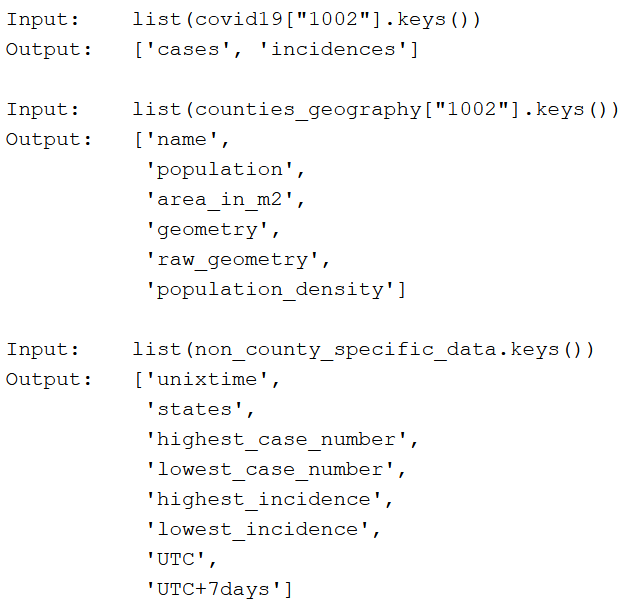
\includegraphics[width=0.8\textwidth]{figures/Durchführung/Dictionarys Bachelorprojekt.png}
    \caption{
    Die Dictionaries non\_county\_specific\_data, counties\_geography und covid19 mit ihren jeweiligen Schlüsseln.
    Für die Dictionaries covid19 und counties\_geography wurde jeweils der Landkreis Kiel (Gemeindeschlüssel 1002) zur Veranschaulichung verwendet.}
    \label{fig:dicts_als_code}
\end{figure}